\documentclass{article} % For LaTeX2e
\usepackage{nips15submit_e,times}
\usepackage{hyperref}
\usepackage{url}
\usepackage{scabby}
\usepackage[numbers]{natbib}

\title{Datasets from Scratch with Online Active Learning}

\author{
Keenon Werling \\
Department of Computer Science\\
Stanford University\\
Stanford, CA 94305\\
\texttt{keenon@stanford.edu} \\
\And
Arun Tejasvi Chaganty \\
Department of Computer Science\\
Stanford University\\
Stanford, CA 94305\\
\texttt{chaganty@cs.stanford.edu} \\
\And
Percy Liang \\
Department of Computer Science\\
Stanford University\\
Stanford, CA 94305\\
\texttt{pliang@cs.stanford.edu}
}

% The \author macro works with any number of authors. There are two commands
% used to separate the names and addresses of multiple authors: \And and \AND.
%
% Using \And between authors leaves it to \LaTeX{} to determine where to break
% the lines. Using \AND forces a linebreak at that point. So, if \LaTeX{}
% puts 3 of 4 authors names on the first line, and the last on the second
% line, try using \AND instead of \And before the third author name.

\newcommand{\fix}{\marginpar{FIX}}
\newcommand{\new}{\marginpar{NEW}}

%\nipsfinalcopy % Uncomment for camera-ready version

\newcommand\pl[1]{\textcolor{red}{[PL: #1]}}

\providecommand{\byt}{\hat{\by}}
\providecommand{\bys}{{\by^*}}
\providecommand{\yt}{\hat{y}}
\providecommand{\ys}{{y^*}}
\providecommand{\Regret}{\operatorname{Regret}}
\providecommand{\p}{p_{\theta}}
\providecommand{\e}{\epsilon}



\begin{document}

\maketitle

\begin{abstract}
What if we could deploy a high-accuracy, real-time classification system, without expensive up-front data labelling?
We describe an ``on-the-job'' classification system, where as queries arrive, we use real-time crowdsourcing to resolve uncertainty where needed and output our prediction when confident.
As the model improves over time, the reliance on crowdsourcing queries decreases. 
We cast our setting as a stochastic game based on Bayesian decision theory, which allows us to balance latency, cost, and accuracy objectives in a principled way.
Computing the optimal policy is intractable, so we develop an approximation based on Monte Carlo Tree Search.
We tested our approach across three tasks---named-entity recognition, sentiment classification,
and image classification.
On the named-entity recognition task, we obtained a 6-7 fold reduction in cost compared to human classification, which requires multiple human votes to achieve the same level of accuracy.
We also achieve a 17\% F1 improvement over taking a single human vote as the answer to each query, and a 28\% F1 improvement over an online learning classifier that cannot query humans.
%Learning with little or no data is an important but understudied problem.
%For most tasks, the current paradigm of first collecting a training dataset and then training a classifier requires a substantial amount of data to be labeled to train a very accurate classifier.
%We propose a  that redistributes the same human effort to achieve
%better results faster: 
%query humans in real time at test time to train a machine learning system {\em
%on the job}.
%%\ac{is it clear what we're doing?}
%%The system only queries humans when it is unsure of its output and learns to 
%Querying humans introduces cost and latency but can improve accuracy over our
%model's prediction.
%We explicitly manage these three key objectives by casting the problem as a
%Bayesian decision theoretic control problem
%and draw on techniques from the game-playing literature.
%The resulting live system provides high quality responses in real-time while
%starting {\em with no training data\/}: we maintain $> 90\%$ F1 consistently on
%a stream of test inputs on the three tasks studied at low cost and latency,
%despite noisy labels from crowd workers.
% outperform baselines?
\end{abstract}

% V1
% Recent work in crowd-powered products has demonstrated the potential of using ``crowd workers'' to power live, low latency systems that accomplish AI complete tasks. 
% These systems suffer from high scaling cost, and the unreliability of workers.
% We propose an \textit{active classification} approach to dramatically reduce the scaling cost and improve the accuracy of such systems.
% In order to also achieve low latency, we investigate \textit{asynchronous} active classification, where multiple requests can be simultaneously ``in-flight.''
% This leads to the twin challenges of how to behave optimally in the presence of asynchronous noisy oracle queries that have not yet returned, and when to return a classification that is ``good enough'' in such a setting.
% We first reduce the problem of optimal asynchronous active classification to a Partial Monitoring game, by making use of Bayesian decision theory.
% We show a bound on achievable regret in this setting, and demonstrate practical heuristics that approach this bound.
% We also show adaptations for traditional Active Learning algorithms to our setting.
% We show empirical demonstration of our proposed algorithms, which demonstrate dramatic improvement over the human-only, machine-only, and baseline human-machine hybrid alternatives in the cost-delay-accuracy tradeoff surface.

% V2?
% Recent work in real-time crowd-powered products has demonstrated the possibility of using human ``crowd workers'' to power live, low latency products that accomplish AI complete tasks. Human-only solutions remain expensive, and do not scale into production. We propose a \textit{active classification} approach to dramatically reduce the scaling cost of such systems, backed by a pool of unreliable crowd-workers. In order to achieve this, we investigate \textit{asynchronous active classification}, where multiple requests can be simultaneously ``in-flight.'' This paper analyzes the \textit{asynchronous requests problem} of how to behave optimally in the presence of asynchronous oracle queries that have not yet returned, and the \textit{optimal stopping problem} of when a classification is ``good enough'' in such a setting. Our solutions to these problems enable a system that shows dramatic improvement over the human-only, machine-only, and baseline human-machine hybrid alternatives in the cost-delay-accuracy tradeoff surface.
% With sufficient labeled data and research effort, supervised learning has been applied in performance critical domains.
% Yet, often logistical/financial constraints mean that data can only be collected and labeled in the presence of a working system, or that insufficient data can be collected to achieve performance requirements.

% V3
% We propose a crowd/machine learning hybrid approach to apply supervised learning in performance critical domains where ``cold start'' barriers exist: we allow our model to query the crowd in real-time {\em at test time}, and learn from the crowd responses online to improve performance and reduce costs on future inputs.
% %Querying humans in real time introduces latency, noise, and cost into the system, which must be minimized.
% Querying humans introduces latency, noise, and cost into the system, which must be minimized.
% We explicitly manage these three key objectives by casting the problem as a Bayesian decision theoretic control problem, and drawing on techniques from game-playing literature for real-time solutions.
% The resulting system provides high quality responses in real-time while starting {\em with no training data\/}: we have achieve $> 90\%$ F1 on the three tasks studied at a low cost, despite noisy crowd worker performance.
% % outperform baselines?


\section{Introduction}

\begin{epigraph}
``It ain't what you don't know that gets you into trouble.\\
It's what you know for sure that just ain't so.'' \\
-- Mark Twain
\end{epigraph}

For the practitioner, supervised learning is largely a solved problem and software to efficiently train classifiers in a variety of domains is readily available.
Yet, adoption remains limited because the deployment of a learning system requires extremely accurate classifiers: mistakes cost business.
The typical solution to this problem is to use more labeled data, which recent crowdsourcing platforms such as Amazon Mechanical Turk or CrowdFlower have made relatively affordable to obtain\findcite{citefest!}.
However, this not only presupposes the ready availability of large amounts of unlabeled data, but also advocates a long, expensive data collection process for uncertain improvements in accuracy.
% This two-stage process fundamentally limits the accuracy we can obtain.
An alternate approach is to use cut out the middle man altogether and use the crowd to label all examples in real-time\cite{cheng2015flock}. 
While this allows us to ensure accurate responses, it becomes prohibitively expensive to scale to more data. 

Our approach interpolates between these two regimes: we query the crowd in real-time when our model is unsure and learn on the crowd responses to improve on future input.
This results in a system that provides users high quality responses in real-time while starting {\em with no training data}.
In this paper, we explicitly address three main challenges that arise in doing so: keeping costs low, guaranteeing low latency and maximizing accuracy.

Let us explore an example use-case for such a framework:
\begin{example*}[Extracting fields from online classifieds]
  \todo{arun: make sexy!}
  You wish to create an online classifieds for apartment listings. 
  Your USP is to automatically identify salient features like the number of bedrooms, housing features, the date of an open house, etc. to allow users to search for listings that match their requirements.
  A successful service will receive thousands of such postings every day, making manual classification impractical.

  Something about starting with zero training data.

  \todo{arun: maybe the rest of the description of the system is in relation to this example}
  Using the system described in this paper, you, the owner, need to specify a model to use - in this case, a linear chain conditional random field is relevant.
  The next challenge is getting data. 
  On each example we can get crowd workers to identify these features, an easy task for people.
  There is a variety of tasks that you can ask people - identifying dates might be easier than not. 
  Could ask people to identify what a particular word, say pool, is.
  Alternatively, you could ask people to identify the nearest landmark.

  This data incorporated into the system to provide a more accurate labeling in the future.
\end{example*}

% Cost and Low-latency
We focus on structured classification problems using conditional exponential families, a general model class that has been used to \todo{citefest}. In such a model, we are given an input, $\bx$, and must predict a number of labels $\by = y_1, \ldots y_n$.

We treat crowd workers as a resource that can provide noisy measurements of some subset of the labels.
Under time and budget constraints, we must optimize over which labels to query when. 
Often, several queries are required on a particular label because of annotator errors by the crowdworker, while at other times it is better to distribute queries across labels.
Similarly, observing a label from one worker lets us decide better which label to query next, but we might not have to time to wait for the response.

We propose an active classification approach using Bayesian decision theory that is able to make these complex behavioral decisions.
This quickly leads to an intractable optimization problem that grows exponentially in complexity with the number of label queries we might ask on a single example.
We propose a novel approximation based on Monte Carlo tree search that retains the behavior of the original Bayesian approach while being computationally tractable.

\todo{(arun): We should make the distinction with active learning much stronger since that's what everyone thinks we're doing. I've moved the related work section to the latter parts because I feel like it's easier to compare our work with existing work given our model.} 

Finally, in practice, labels from crowd workers are often inaccurate.
We use the measurements framework of Liang et.\ al\cite{liang09measurements} to incorporate noisy responses from crowdworkers in our model.
Having an accurate estimate of the error rates for crowd workers is essential to accurately predicting how many queries are required.
Prior work\findcite{unsupervised crowd labeling} uses inter-annotator agreement to predict per-user error rates in an unsupervised manner. 
The online nature of our task limits the number of responses we have on the same label.
Instead, we learn the error rates in an unsupervised fashion using online EM, which also allows us to incorporate unlabeled data.

% Experiments
We evaluate our system on four different tasks: named entity recognition, information extraction from user generated content, image classification and sentiment classification on tweets.
We show that by querying crowdworkers at classification time, we can significantly outperform a system trained on fully labeled data, for a fraction of the cost of the baseline of asking crowdworkers for labels for each example, as well as the system trained on fully labeled past data.
On X of the Y tasks, we produce a classifier comparable with the state of the art while obtaining a much smaller subset of the training labels noisily from the crowd. 
In fact, we are comparable with state of the art-ish with a handful of the training labels.
An open-source implementation of our system will be made available.

% Recent work has shown that it is possible to use real-time on-demand workers to power everything from AI-complete email clients~\cite{kokkalis2013emailvalet} to real-time activity surveillance and classification~\cite{lasecki2013real}.
% These purely crowd-based solutions are prohibitively expensive at scale.
% Powering the crowd-based email client \textit{EmailValet}~\cite{kokkalis2013emailvalet} for a single end user for a year costs over \$400.
% 
% These systems typically work by ``pooling'' on-demand workers from high latency job-posting platforms like Amazon Mechanical Turk or CrowdFlower on a website designed by the system architect~\cite{lasecki2011real}.
%  The ``pooling'' process can take several minutes, but once in place the workers can be queried at very low latencies by pushing requests to their web-browsers.
%  This pool of workers can demonstrate high rates of turnover, and unreliability amongst individual annotators.
% 
% Existing systems query this pool directly, allowing for annotator noise by incorporating consensus building systems like voting and chat.
% 
% 
% Active classification~\cite{greiner2002learning}, a close sibling of active learning, is a setting in which a classifier is allowed to query for more information, at some cost, before turning in classifications.
%  This active classifier is intended to reduce its need for costly, slow human labels over time by learning from past observations.
%  We propose to adapt the active classification framework to the pooled-worker setting to query this pool more cheaply, accurately, and quickly, without sacrificing the advantages live of crowd-powered interfaces.
% 
% Previous work in online active learning (which is closely related to what we're proposing) has focused on multi-class classification (\cite{chu2011unbiased},~\cite{agarwal2013selective},~\cite{cheng2013feedback},~\cite{vzliobaite2011active},~\cite{helmbold1997some}).
%  Multi-class classification is an insufficiently rich primitive to handle many of the tasks that crowd-workers are enabling in existing systems, like information extraction or object detection.
%  Instead, we will build our platform around arbitrary log-linear markov network classification, where we assume it is possible to query workers for opinions on individual nodes.
%  Thus each ``active classification'' in our proposed setting is instantiate with a markov network and involves using model priors trained on previously seen data to choose to query the worker-pool for opinions about nodes, and then returning a classification informed by those opinions.
% 
% 
% This setting poses several distinct challenges that have not been sufficiently addressed in previous literature.
%  We need to be sensitive to time delays, returning results at least as quickly as the pure-crowd baseline we intend to improve upon.
%  We also need to be sensitive to inaccurate oracles.
%  These two criteria, in the pooled-worker setting, means that we need an active classifier who is able to hide latencies of redundant queries by launching them \textit{asynchronously}.
%  This leads to the two challenges we will address in this paper, which can both be clustered under \textit{optimal asynchronous behavior}: we need to be able to handle the decision to ask for another query or turn in existing results in the presence of ``in-flight requests,'' which can fail due to worker turnover, where our loss term is sensitive to time delay.
%  We draw inspiration from work in Bayesian Active Learning to tackle these problems.




\section{Model}
\label{sec:model}

\begin{figure}
  \begin{centering}
    \begin{subfigure}[b]{0.58\textwidth}
      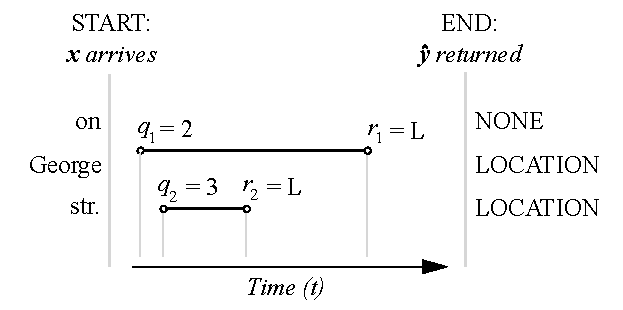
\includegraphics[width=\textwidth]{figures/piano-roll.pdf}
      \caption{Structured prediction behavior over time}
    \end{subfigure}
    \hfill
    \begin{subfigure}[b]{0.38\textwidth}
      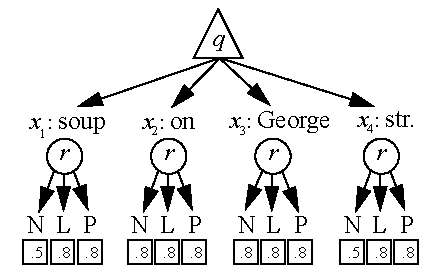
\includegraphics[width=\textwidth,height=0.23\textheight,keepaspectratio]{figures/single-move.pdf}\\[1.7ex]
      \caption{Single-query game tree}
    \end{subfigure}
  \end{centering}
\caption{Example behavior while running structure prediction on the tweet ``Soup on George str.''
We omit the \scres{} from the game tree for visual clarity.
}
\label{fig:game-tree}
\end{figure}


% ARUN: This is a little too much detail too early.  
% Define game top-down
% We define a stochastic game with two players, the system and the crowd.
% The system gets ``woken up'' every time something in the environment changes, and is allowed to make a move.
% The game starts with a $\bx$ arriving in need of a label, and the system must make a decision.
% Possible decisions are TURN\_IN, WAIT, and launching a query $q_0$ on one of the variables $\by_i$.
% If the system decides to TURN\_IN, the best guess $P_{\theta}(\bx|\by)$


% High-level what is the game?
We model on-the-job learning as a stochastic game with two players: the system and the crowd.
The game starts by the system receiving input $\bx$ and ends when the system turns in a set of labels $\by = (y_1, \ldots, y_n)$. 
During the system's turn, the system may choose an action $q \in \{1, \ldots, n\}$ to ask the crowd to label $y_q$. 
The system may also choose 
the wait action ($q = \acwait$) to wait for the crowd to respond to any pending queries
or
the return action ($q = \acret$) to terminate the game and return its best estimate given responses received so.\footnote{When $q = \acwait$ or $q = \acret$, $y_q$ is not defined and is ignored.}
The system takes as many turns in a row as it wants, before deciding to wait or turn in.
When the wait action is chosen, the turn switches to the crowd, which provides a response $r$ to one pending query, and advances the game clock by a random amount (human query latency).
The turn then immediately reverts back to the system.
The key challenge is to determine which action the system should take during its turn.
For this, we appeal to Bayesian decision theory.

% How is the game played? maximizing utility under the model, which will be subsequently.
Under Bayesian decision theory, the \emph{optimal choice} of actions $\bq = (q_1, \ldots, q_k)$ for the system is the set of actions that attain the maximum expected utility (i.e.\ value) for the game:
\begin{align}
  \label{eqn:value}
V^* = \max_{\bq} \E_{p(\br \mid \bx, \bq)}[U(\bq, \br)],
\end{align}
where $\br = (r_1, \ldots, r_k)$ are the responses to the queries, $p(\br \mid \bx, \bq)$ is the system's model of the environment and $U(\bq, \br)$ is the utility which captures the cost of making the queries and the accuracy of the predictions given the responses. 
We will define these latter two quantities next.
%We will define these latter two quantities after looking at the example below:

%The \emph{value} of the game is the maximum expected utility:
%\begin{align}
%  V^* = \max_q \E_{p(r \mid \bx, q)}[U(q, r)],
%\end{align}
%and the \emph{optimal policy} is to choose the action $q$ that attains $V^*$.

% Arun: I don't think this is very useful -V
%Note that the system computes the $V^*$ by only \emph{simulating} possible futures, not by actually querying the crowd.

% Example time!
%Let us look at the example in \figureref{game-tree} more intuitively:
%querying one of the end positions ($q = 1$ or $q = 4$),
%is less informative than choosing the middle positions ($q = 2$ or $q = 3$),
%assuming the model propagates information between adjacent positions.
%Indeed, the expected utilities with a uniform distribution over $r$
%are $0.7$, $0.8$, $0.8$, and $0.7$, respectively, and so both $q = 2$ and $q = 3$ are optimal actions.

%Note that the system computes the $V^*$ by only \emph{simulating} possible futures, not actually querying the crowd.
%The simulation is based on the transition probabilities $p(r \mid \bx, q)$ and the utilities $U(q, r)$, which are based on a probabilistic model that connects input, output, responses, and time delays.

% Start model.
\paragraph{Environment model.}

We now define the model of the environment that the agent uses.
Given input $\bx$ and queries $\bq = (q_1, \dots, q_k)$ issued at times $\bs = (s_1, \dots, s_k)$,
we define a distribution over the output $\by$, responses $\br = (r_1, \dots, r_k)$
and response times $\bt = (t_1, \dots, t_k)$ as follows:
\begin{align}
  \label{eqn:dynamics}
%p(\by, \br, \bt \mid \bx, \bq) \eqdef \p(\by \given \bx) \prod_{i=1}^k \presp(r_i \mid \bx, \by, q_i) \ptime(t_i \mid \bx, \by, q_i, s_i).
p(\by, \br, \bt \mid \bx, \bq) \eqdef \p(\by \given \bx) \prod_{i=1}^k \presp(r_i \mid y_{q_i}) \ptime(t_i \mid s_i).
\end{align}
The three components, specified by the user, are as follows:
First, $\p(\by \given \bx)$ is the \emph{prediction model} (e.g.\ a standard linear-chain CRF).
Second, $\presp(r \given y_q)$ is the \emph{response model} which describes the distribution of the crowd's response $r$ for a given a query $q$ when the true answer is $y_q$.
%
If the crowd workers were infallible we could define $\presp(r \given y_q)$ to be $1$ iff $r = y_q$, but annotation errors are typical in practice. 
In our experiments, we model $\presp(r \given y_q)$ using $\presp(r \given y_q) = 0.7$ iff $r = y_q$\footnote{ We found the humans we hired were roughly 70\% accurate in our experiments}, and distribute the remaining probability for $r$ uniformly.
%
Finally, $\ptime(t \given s)$ is the \emph{time delay model}, which governs how long a given query $q$ will take. While, in reality, $t$ depends on many factors including the input, in the interest of simplicity we assume $t - s$ to be drawn from a gamma distribution with globally fixed parameters.\footnote{
Of course, both $\presp$ and $\ptime$ can easily be extended to depend arbitrarily on the input $\bx$.}
We also define the \emph{response at time $\tau$}, $r[\tau]$, to be $r$ if $\tau > t$ and $\emptyset$ otherwise.

% Doing things with the model
Given this full model, we can compute $p(\br \mid \bx, \bq)$ simply by marginalizing out $\by$ and $\bt$ from \equationref{dynamics}.
We can also compute the distribution over responses at a particular time $\tau$, $p(\br[\tau] \given \bx, \bq)$, where $\br[\tau] = (r_1[\tau], \ldots, r_k[\tau])$.
% Describe the simplifications on how time is moved forward, with possibly an example

\paragraph{Utility.}

%The simulation dynamics model defines the transition probabilities of the game through various conditioning and marginalization operations.
We now define the utility of the game at time $\tau$, which must trade off two things.
The first is the accuracy of the MAP estimate according to the model's best guess of $\by$ incorporating all responses received by time $\tau$.
The second is the cost of making queries: a (monetary) cost $\weightmoney$ per query made and penalty of $\weighttime$ per unit of time taken.
Formally, the utility is defined as follows:
\begin{align}
  \label{eqn:utility}
  U_\tau(\bq, \bs, \br, \bt) &\eqdef F(p(\by \given \bx, \bq, \bs, \br[\tau], \bt)) - (k \weightmoney + \tau \weighttime), \\
  F(q) &= \E_{q(\by)}[\accuracy(\arg\max_{\by'} q(\by'))].
\end{align}

\equationref{utility} is related to \equationref{value} by considering the utility at the time of the last request, $\tmax = \max\{t_1, \ldots, t_k\}$: $U(\bq, \bs, \br) = \E_{\bt}[U_{\tmax}(\bq, \bs, \br, \bt)]$.
In practice, we actually consider the utility at the earlier of $\tmax$ and a specified time limit to respond, $\deadline$.

%Importantly, we are only conditioning on the responses $\br[t]$ that are available at time $t$.

% Behavior!
\paragraph{Behavior.}
Let's look at typical behavior that we expect the model and utility to capture.
Firstly, because the system wants to maximize the accuracy while minimizing the number of queries, it will prioritize asking queries that provide the most information.
For example,
in the model in \figureref{game-tree}, the model, a linear-chain CRF, propagates information between adjacent labels. 
Thus, querying one of the middle positions ($q = 2$ or $q = 3$) can be more informative than one of the end positions ($q = 1$ or $q = 4$).
Indeed, this is reflected in the expected utilities of each query: with a uniform distribution over the responses, they are $0.7$, $0.8$, $0.8$, and $0.7$ respectively. Thus, both $q = 2$ and $q = 3$ are optimal actions. \todo{This is a really lame example with poor intuition.}

We also expect the system to be able to use queries judiciously when the cost per query, $\weightmoney$, is much larger than the cost per unit time, $\weighttime$.
For example,
if we had already made one query $q_1$ and gotten a response $r_1$,
we can incorporate the evidence, which will propagate through the CRF
and inform the distribution over possible responses $r_2$ for the next query $q_2$:
$p(r_2 \mid \bx, q_1, r_1, q_2)$.
We see this happen \todo{example!}

%If we had already made one query $q_1$ and gotten a response $r_1$,
%we can incorporate the evidence, which will propagate through the CRF
%and inform the distribution over possible responses $r_2$ for the next query $q_2$:
%$p(r_2 \mid \bx, q_1, r_1, q_2)$.
%
%\todo{WEIRD}
%The temporal aspect of the model also allows for interesting possibilities
%and is important for handling asynchronous queries and responses.
%Suppose we made a query $q_1$ at time $s_1$ but have not yet gotten response $r_1$.
%We might still want to ask for various probabilities \emph{at time} $t$,
%which involves integrating over possible future responses $r_1$ and response times $t_1$.
%Formally, define $r_i[t]$ to be the response at time $t$, which is equal to $r_i$ if $t_i \le t$
%or $\emptyset$ if $t_i > t$.
%Then we could ask about the probability of a response $r_2$ at time $t$,
%which integrates over the possibility of having received $r_1$ or not:
%\begin{align}
%p(r_2[t] \mid \bx, q_1, q_2) = p(t_1 \le t \mid s_1) p(r_2[t] \mid \bx, q_1, r_1, q_2) + p(t_1 > t \mid s_1) p(r_2[t] \mid \bx, q_2).
%\end{align}
%
%Let us revisit the example in \figureref{game-tree} by looking at the game tree on the right where the system turns in an answer after a single query.
%The square leaf nodes store the value of obtaining responses for each query.
%Intuitively, because the model (a linear-chain CRF) propagates information between adjacent labels, querying one of the end positions ($q = 1$ or $q = 4$) is less informative than the middle positions ($q = 2$ or $q = 3$).
%Indeed, this is reflected in the expected utilities of each query: with a uniform distribution over the responses, they are $0.7$, $0.8$, $0.8$, and $0.7$ respectively. Thus, both $q = 2$ and $q = 3$ are optimal actions.
%\todo{this is a bit of a lame example.}

\section{Game playing.}
\label{sec:game-playing}

In \sectionref{model} we modeled on-the-job learning as a stochastic game played by the system, and defined a reasonable model of the environment and utility for the system to maximize.
We now turn to the problem of finding a policy that maximizes the expected utility, which is, of course, intractable due to the large state space and continuous time\reword.
We propose an approximate Monte Carlo algorithm based on Monte Carlo tree search with progressive widening (to handle continuous time) and TD-learning (to handle the large state space).


%Having defined the simulation dynamics and utility, we can now define the full game tree,
%which is an extension of our initial example in \figureref{game-tree}~(right).
%The technical challenge here is to incorporate the modeling of continuous time
%into a traditionally discrete game tree.
%A naive approach might be to discretize time and treat each level of the game
%tree as a time step, but this discretization is inefficient.
%Our strategy is to consider only represent game states corresponding to pivotal times $t$
%and model waiting times as random actions played by the crowd.
%%\citep{guo2009continuous}

% Game state, abstract goal
First, we begin by describing how the system simulates the game.
Formally, a \emph{game state} $s = (\now, \bq, \bs, \br, \bt)$
consists of the current time $t$, the queries $\bq$ issued at time $\bs$,
responses $\br$ that have be received at time $\bt$.
We assume that all queries $q_1, \dots, q_{k-1}$ have been issued,
but the last query $q_k$ has yet to be;
and some subset of responses in $r_1, \dots, r_{k-1}$ have been received,
and the rest are ``in flight.''
We focus on the problem of deciding (i) what to query ($q_k$)
and (ii) when to query ($s_k$) to maximize expected utility
at some future $\deadline$ (see \figureref{game-tree}~(left) for reference).
Recall the intuition: if $\deadline$ is near, then we would want to query
many labels in parallel; otherwise, we should operate more sequentially,
so as to be more adaptive.

% Describe game tree
At each state $s$ in the game tree in which it is the system's turn,
we query a position $q_k \in \{1, \dots, n\}$ (not necessarily new)
or wait until ($q_k = \emptyset$);
the successor state simply incorporates $q_k$.
If it is the crowd's turn,
then we sample the time of the first ``in flight'' response along with its value.
Formally, let $F = \{ 1 \le j \le k-1 : q_j \neq \emptyset \wedge r_j = \emptyset \}$ be the ``in flight'' queries.
Sample $t_j$ according to the time delay model for each $j \in F$
and take the earliest event $j^* = \arg\min_{j \in F} t_j$;
the actual response $r_{j^*}$ is drawn independently from the dynamics model conditioned on the queries and responses
in the state $s$;
the successor state incorporates $r_{j^*}$ and $t_{j^*}$ and advances time from $\now$ to $t_{j^*}$.
Technically, the optimal strategy might be to wait for an intermediate amount of time before $t_{j^*}$,
so our restriction to considering decisions only at response times is an approximation.

The following example shows one path over the states of the game tree corresponding to \figureref{game-tree}~(left),
where the system takes action $q_2 = 4$ (labeling \nl{str.}) and then the crowd responds
at time $1.7$ with $r_2 = \scloc$.
Note that the response $r_1$ for $q_1 = 3$ (\nl{George}) is still pending.
\begin{center}
\begin{tabular}{|ll|}
  \hline $\now = 1$ & \\
  \hline
  $q_1 = 3$         & $q_2 = \emptyset$ \\
  $r_1 = \emptyset$ & $r_2 = \emptyset$ \\
  \hline
\end{tabular}
$\stackrel{\text{\small system}}{\implies}$
\begin{tabular}{|ll|}
  \hline $\now = 1$ & \\
  \hline
  $q_1 = 3$         & $q_2 = 4$ \\
  $r_1 = \emptyset$ & $r_2 = \emptyset$ \\
  \hline
\end{tabular}
$\stackrel{\text{\small crowd}}{\implies}$
\begin{tabular}{|ll|}
  \hline $\now = 1.7$ & \\
  \hline
  $q_1 = 3$         & $q_2 = 4$ \\
  $r_1 = \emptyset$ & $r_2 = \text{\scloc}$ \\
  \hline
\end{tabular}
\end{center}

%\paragraph{Prediction model.}
% PL: form isn't relevant here since later we use other types of models anyway
%Assume our model
%We consider the family of conditional random fields
%exponential models, a popular class of models that include logistic regression
%and conditional random fields.
%Let $\bx$ be a given input, then the labels $\by = y_1, \ldots, y_n \in \{1,
%\dots, L\}$ are generated by the following conditional distribution:
%\begin{align*}
%  \p(\by \given \bx) 
%  &\propto \exp(\theta^\top \phi(\bx, \by)),
%\end{align*}
%where $\phi(\bx, \by)$ are features
%and $\theta$ are model parameters.
%In this paper, $\p(\by \given \bx) We assume that inference is efficient, which it is
%for our chain-structured models.
%(e.g.\ $\phi$ factorizes over the
%labels $\by$) or otherwise admits efficient marginal computation.

%For example, the model in \figureref{crf} is a linear-chain conditional random
%field. The input is the sequence of words in the tweet and the output is a
%label in the set \scnone, \scres, \scloc{} and \scper. Marginal inference can
%be efficiently computed using the Viterbi algorithm.

%Conventionally, we are given a training dataset $\sD = \{\bx_i, \by_i\}$ and can learn $\theta$ by optimizing the convex log-likelihood objective $\sL(\theta) = \sum_{t=1}^T \log \p(\by\oft{t} \given \bx\oft{t})$.
%In our setting, however, we do not observe the gold labels $\by$. 
%Instead, we can ask the crowd to provide a ``measurement'' for some subset of the labels.
%Let $\Sigma = \{\sigma_i\}$ be the set of possible measurements we can ask the crowd for and 
%let $\by_\sigma \subseteq \by$ be the subset of labels queried.

%\paragraph{Response model.}
%Let $q \in \{1, \ldots, n\}$ be a query on for the label $y_q$.
%We model the response, $r$, with an exponential measurement model:
%\begin{align*}
%  p_\beta(r \given x, y, q) 
%  &\propto \exp \left( \beta^\top\psi(\bx, y_q, r) \right),
%\end{align*}
%where $\beta$ and $\psi$ are extra parameters and features for the human error model. 
%%The choice of an exponential model allows us to simply include measurements as an additional factor.
%\figureref{crf}(c) shows the original graph with additional measurement nodes.
%A simple human error model is to return the true label with probability $1-\epsilon$ and a random label otherwise.
%In our running example, some classes, e.g.\ $\textsc{none}$, are more easily identified than others: in this setting responses can be modeled to be sampled from a confusion matrix.
%
%Finally, we model delay to be drawn from a Gamma distribution: $\tau \sim \Gamma$\footnote{We assume here for simplicity that the response delays are independent of the input and which label is being queried. The model can easily be generalized to incorporate these settings.}.
%\ac{The gamma is missing parameters.}
%Note that the total time taken on a prediction, $t$, depends not only on how many requests are made, but also when they are scheduled.
%%We study the problem of how to best schedule multiple requests in \sectionref{async}.
%
%Next, we describe how we use our models to predict labels and learn from partial feedback.

%\paragraph{Making predictions.}
%Given parameters $\theta, \beta$ and responses $r_1, \ldots, r_m$, our model makes predictions using maximum likelihood:
%$\byt \given \bx, r_1, \ldots r_m = \argmax_{\by} \p(\by \given \bx, r_1, \ldots r_m)$.
%
%\paragraph{Learning from responses.}
%Recall that we do not have gold labels for our data, but only noisy measurements: we do not have supervised examples to learn from. 
%As a simple heuristic, we use the output from our model as gold labels and update our parameters $\theta$ periodically.  
%We consider the response parameters $\beta$ to be fixed a priori.
%The time delay parameters can easily be estimated from the observed response delays.
%%In future work, we plan to explore using (online) expectation-maximization to jointly learn parameters for our model and the human error model in an unsupervised fashion.
%
%\paragraph{Computing expected utility.}
%
%\ac{Text}
%We cast this problem in the Bayesian decision theoretic framework: our objective is to maximize our expected utility under our current model,
%$\p(\by \given \bx, \br)$:
%\begin{align*}
%  u &= \E_{\by \sim \p(\cdot \given \bx, \br)}[1 - \ell(\by, \byt) + C(\bq, t)].
%\end{align*}


\section{Evaluation}
\label{sec:eval}


\bibliographystyle{unsrtnat}
\bibliography{all}

\end{document}
